
\section{Architecture}
\label{sec:architecture}

The distributed and decentralized \textsc{c}ollabo\textsc{rat}ive
\textsc{e}ditor \CRATE\footnote{\url{https://github.com/Chat-Wane/CRATE}}
comprises four layers:
\begin{inparaenum}[(i)]
\item the graphical user interface that renders the document to the users
  (cf. Figure~\ref{img:screenshot});
\item the sequence structure layer that represents the local replica of the
  document (cf. §\ref{sec:structure});
\item the causality layer that tracks semantic causality between operations,
  e.g., the removal of a character cannot precede its insertion.
\item the network layer that both builds a network of browsers and use it to
  disseminate the operations performed on documents (cf. §\ref{sec:network});
\end{inparaenum}

\begin{figure*}
  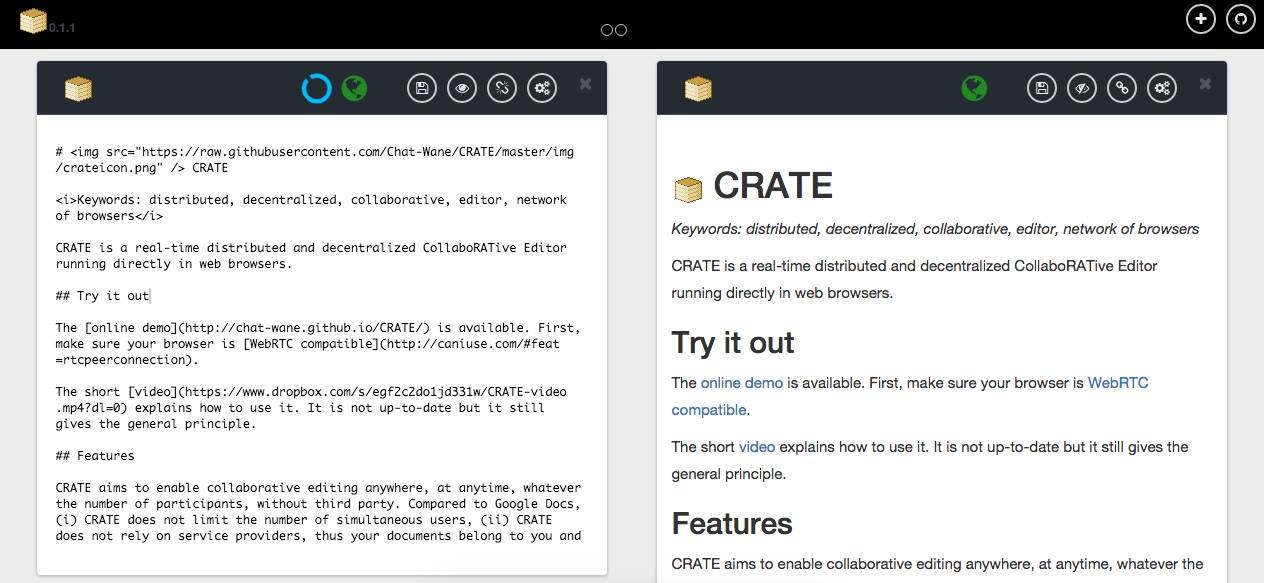
\includegraphics[width=\textwidth]{./img/screenshot.png}
  \caption{\label{img:screenshot} \CRATE screenshot}
\end{figure*}


%%% Local Variables:
%%% mode: latex
%%% TeX-master: "../paper"
%%% End:
